\section{Background}                     % context and prior work the project builds on
\label{sec:background}                   % \secref{sec:background}

This section recalls the scientific context,
how the data were collected, how the existing point cloud was produced from them, and which part
of the data that work left unused.

% ------------------------------------------------------------------------------
\subsection{Karst conduits and the RKE project}   % why these environments are studied
\label{sec:bg_context}                            % \secref{sec:bg_context}

Karst systems form when water dissolves soluble rock such as limestone, creating networks of
underground caves and conduits \citep{ford2007karst}. They store the groundwater used by about a
quarter of the world's population \citep{goldscheider2020karst}. They are also a hazard: water
moves through the conduits quickly and with little filtering, so pollution spreads fast, and
heavy rain can overwhelm the network and cause sudden floods. Modelling and managing such an aquifer
requires knowing the geometry of its conduits, yet many of them are out of reach for human divers.
The \emph{Robots for Karst Exploration} (RKE) project therefore develops robotic operations to map
these flooded networks \citep{lapierre2021karst}.

% ------------------------------------------------------------------------------
\subsection{Data acquisition}            % the platform and its sensors
\label{sec:bg_acquisition}               % \secref{sec:bg_acquisition}

The data were recorded in March~2023 in the flooded conduit of the Fontaine de N\^imes with the
NavScoot~2, a diver-propelled vehicle carrying the sensor suite (Figure~\ref{fig:bg_navscoot}). Its sensors serve two purposes. For
navigation, a Doppler velocity log (DVL, Nortek DVL~1000) measures the velocity of the vehicle, an
inertial measurement unit (IMU, SBG Ellipse~A) its orientation and a pressure sensor (Blue Robotics
Bar30) its depth, while a forward-looking echosounder (ISA~500) carries its own attitude unit. For
mapping, the vehicle carries two mechanically scanned imaging sonars (MSIS). The \emph{vertical}
profiling sonar (Tritech Super SeaKing, beam width 1--2$^\circ$) sweeps a plane across the conduit
and measures its cross-section. The \emph{horizontal} scanning sonar (Blue
Robotics Ping360) sweeps a full circle in the horizontal plane, with a beam 2$^\circ$ wide
horizontally but 25$^\circ$ high vertically. An MSIS emits one narrow acoustic ping at a time and
rotates its head step by step; each ping returns an intensity profile along a single direction
(the \emph{echo}). A full scan is therefore built over several seconds while the vehicle keeps
moving.

\begin{figure}[!htbp]                    % the acquisition platform
  \centering
  \begin{minipage}[b]{0.48\linewidth}    % left: the vehicle
    \centering
    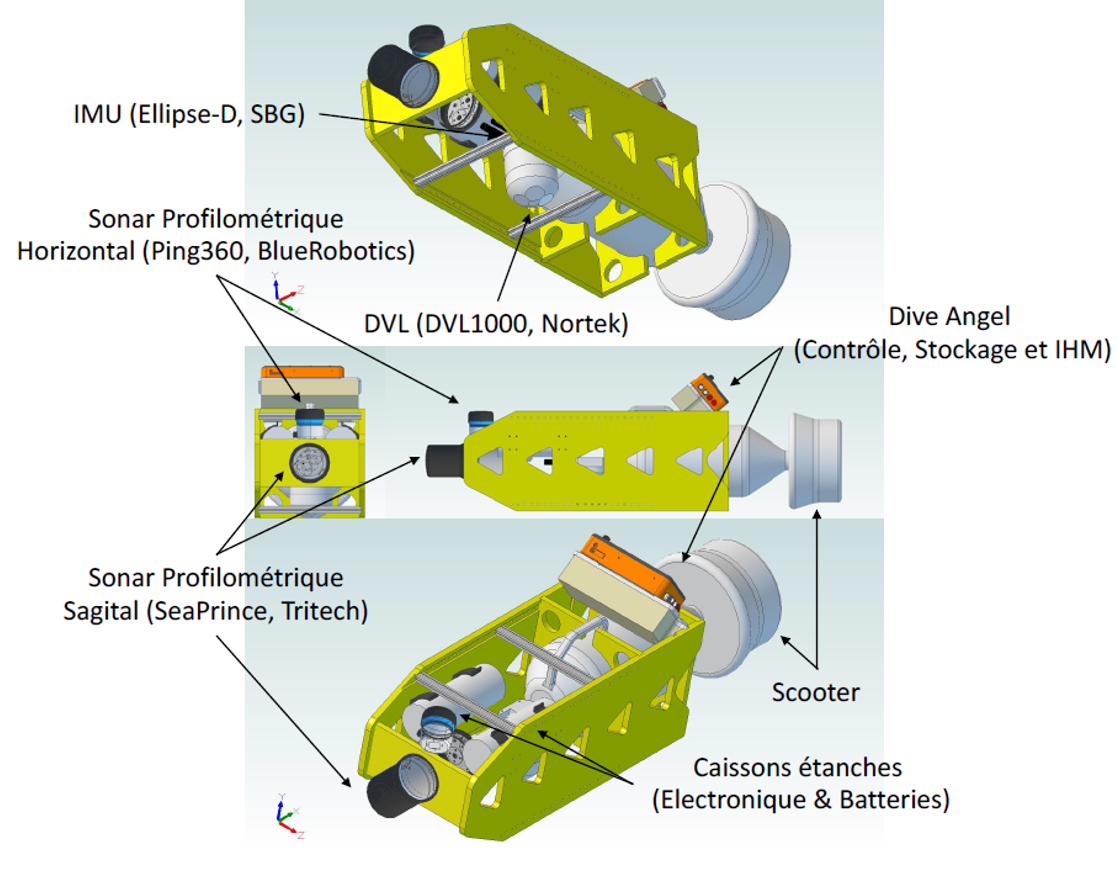
\includegraphics[width=\linewidth, height=5cm, keepaspectratio]{figures/Scooter.png}\\[0.3em]
    {\small (a)}
  \end{minipage}\hfill
  \begin{minipage}[b]{0.48\linewidth}    % right: the diver operating it
    \centering
    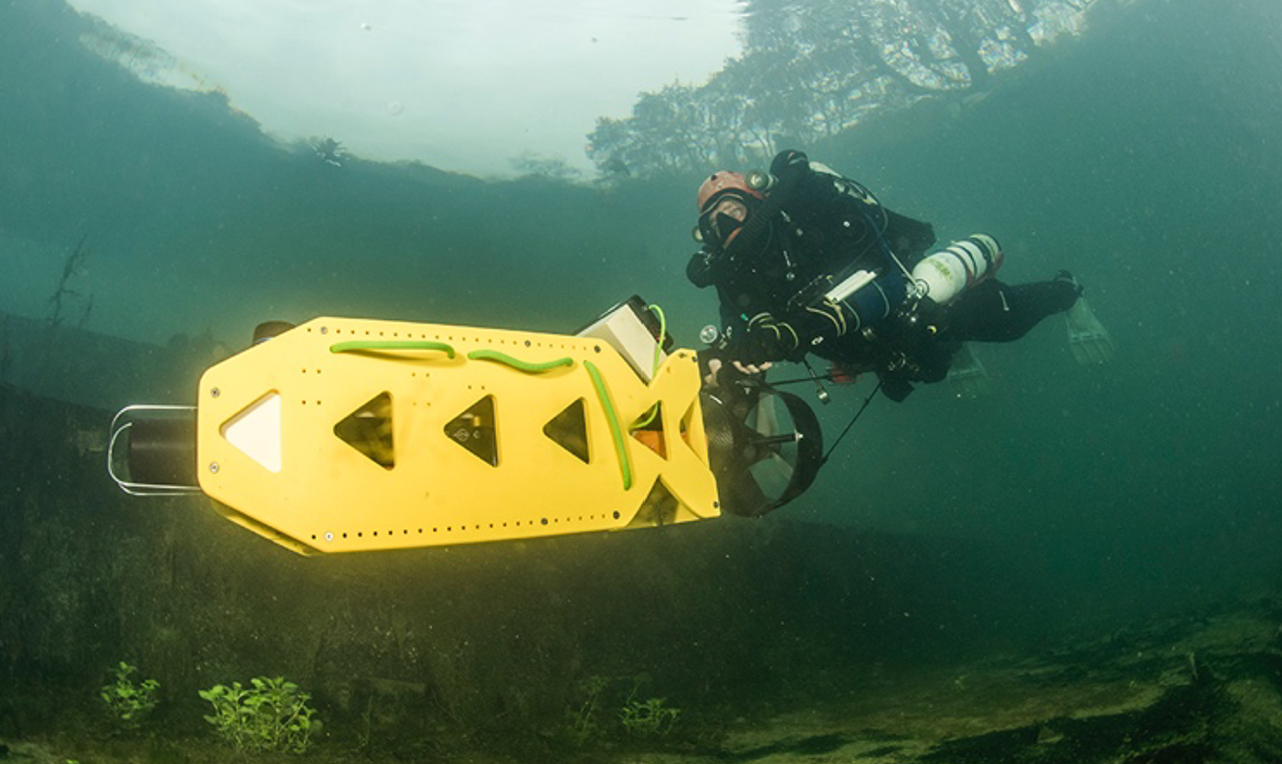
\includegraphics[width=\linewidth, height=5cm, keepaspectratio]{figures/Scooter_diver.png}\\[0.3em]
    {\small (b)}
  \end{minipage}
  \caption{The NavScoot~2 acquisition platform \citep{margaritis2025internship}: (a) the vehicle
           with its sensors; (b) the diver operating it.}
  \label{fig:bg_navscoot}
\end{figure}
% ------------------------------------------------------------------------------
\subsection{From raw data to a point cloud}  % the existing pipeline
\label{sec:bg_pipeline}                      % \secref{sec:bg_pipeline}

In the previous work \citep{margaritis2025internship}, the trajectory of the NavScoot~2 was
first estimated by dead reckoning, integrating the DVL velocity rotated by the IMU orientation,
with the depth sensor giving the vertical position. In every ping of the vertical sonar, the first
strong return was kept as the distance to the wall and placed in 3D with the pose of the vehicle at
that time, giving a point cloud of about 50\,000 points (Figure~\ref{fig:bg_pointcloud}). The drift
accumulated by the trajectory was then reduced with Continuous-time SLAM
\citep{ nuchter2017cartographer}.

\begin{figure}[!htbp]                    % the data this project starts from
  \centering
  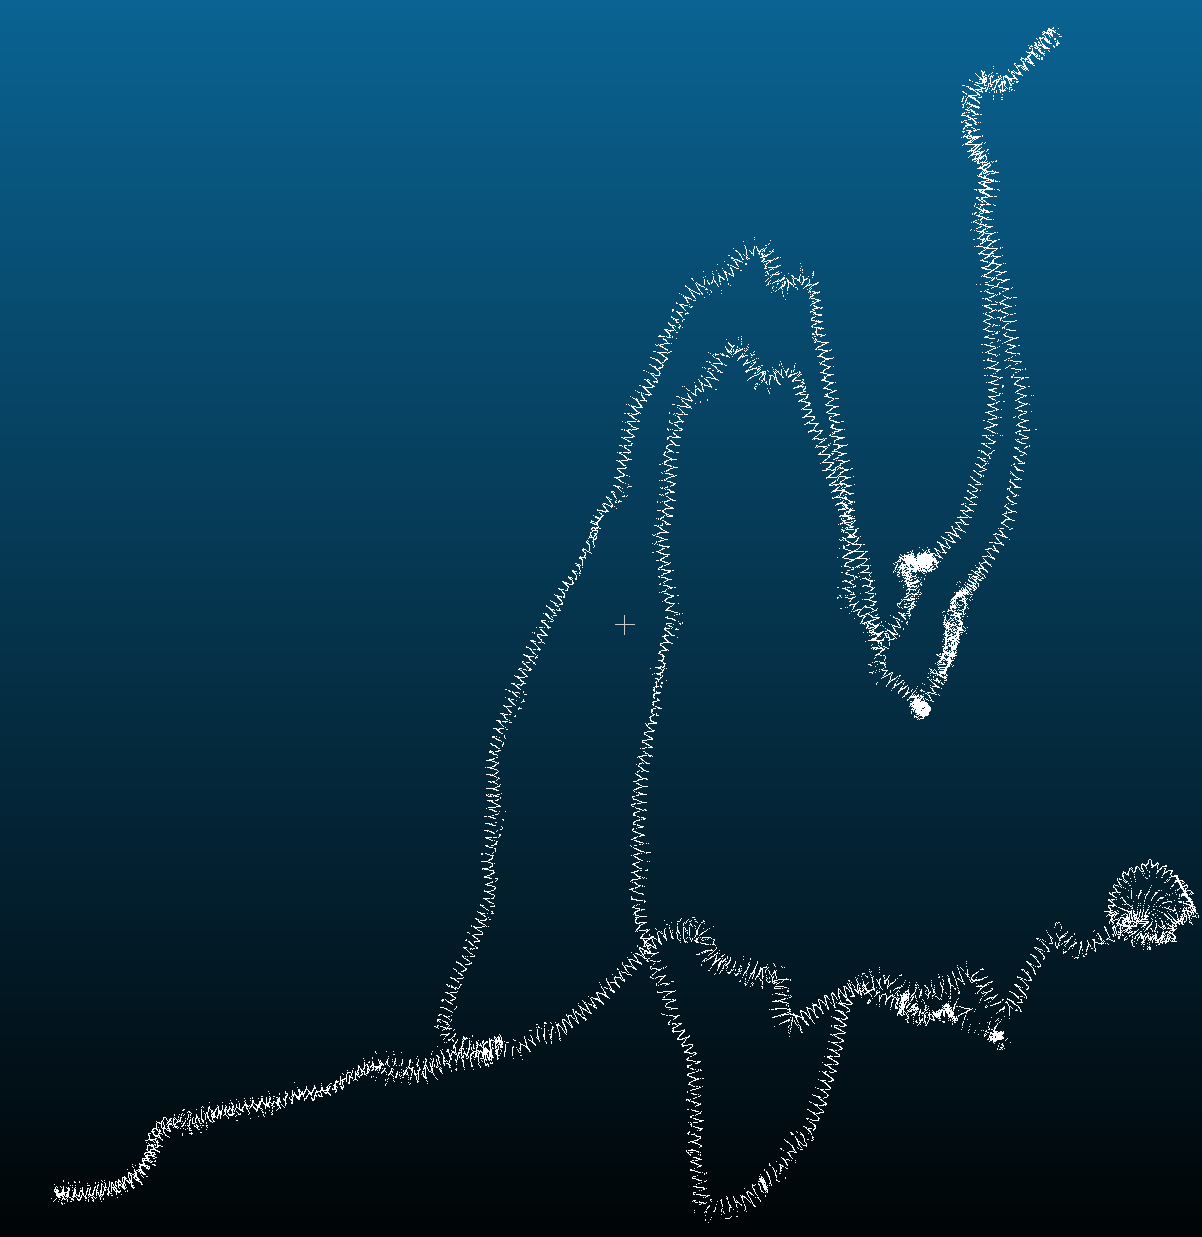
\includegraphics[width=0.9\linewidth, height=9cm, keepaspectratio]{figures/initial_point_cloud.png}
  \caption{Initial point cloud of the conduit obtained from the vertical sonar \citep{margaritis2025internship}.}
  \label{fig:bg_pointcloud}
\end{figure}

% ------------------------------------------------------------------------------
\subsection{The unused horizontal sonar}  % the gap this project addresses
\label{sec:bg_gap}                        % \secref{sec:bg_gap}

The point cloud of \citet{margaritis2025internship}, and everything built on it, uses only the
echoes of the vertical sonar. Each vertical scan describes one cross-section of the conduit, so
the map is a sequence of slices whose spacing along the conduit depends entirely on the estimated
trajectory. The horizontal sonar, recorded during the same dive, sees the walls along the
direction of travel (Figure~\ref{fig:bg_scanplanes}) and could provide extra information about the
geometry of the conduit, but it was not used in that work. Exploiting it is not trivial. With a
beam 25$^\circ$ high, an echo may come from anywhere within that vertical aperture, so the height
of each detected point is uncertain. A 360$^\circ$ sweep also takes several seconds, during which
the vehicle moves and turns, so each ping must be placed with its own pose. Finally, the two sonars
observe perpendicular planes, at different rates and with different noise, and their measurements
must be expressed consistently in a single frame and point cloud. The aim of this project is to
process the horizontal sonar data and merge them with the vertical sonar data into one consistent
point cloud as proposed in the work of \citet{breux2020elevation} with the only difference that in this work we will apply the the method in real data, where \citet{breux2020elevation} 
applied it in simulated data and in our best of our knowledge this is the first time it is applied to real data.

\begin{figure}[!htbp]                    % geometry of the two scanning planes
  \centering
  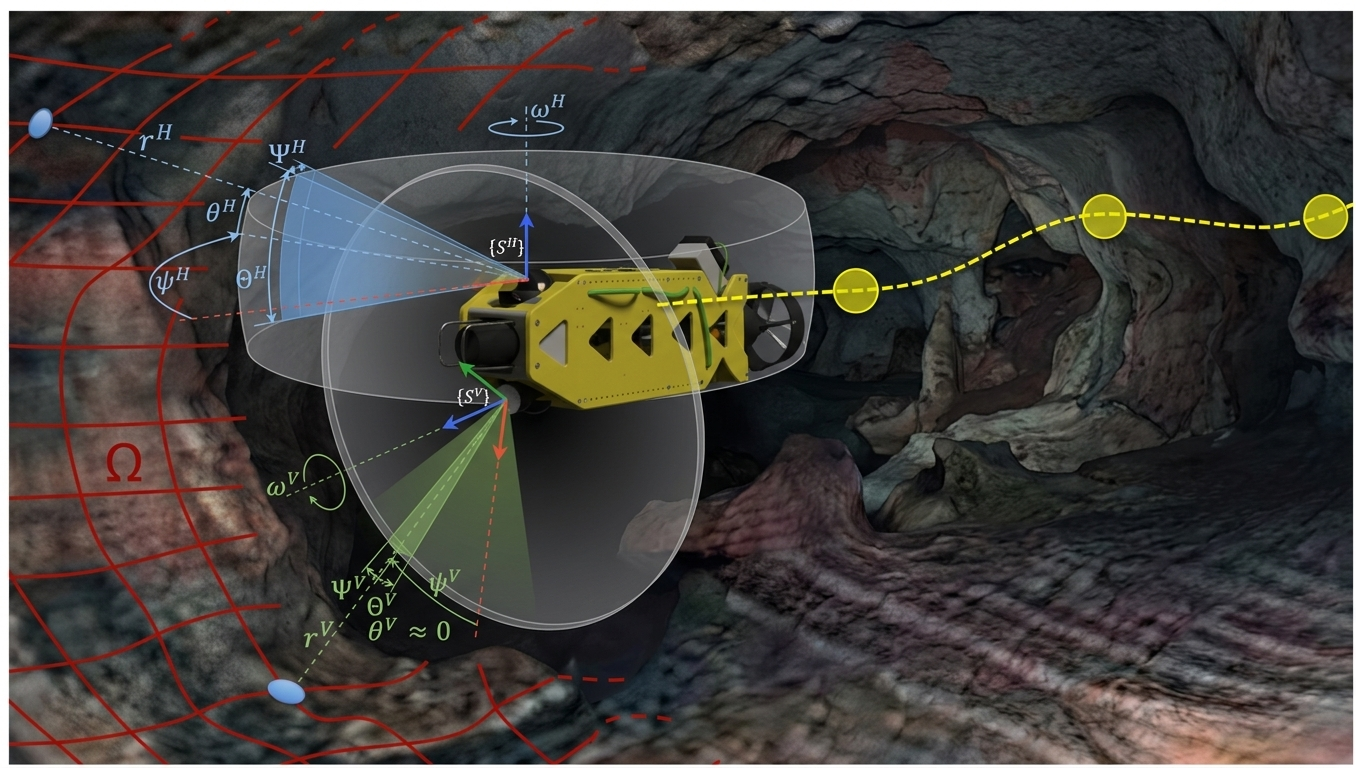
\includegraphics[width=0.9\linewidth, height=9cm, keepaspectratio]{figures/scanning_planes.jpeg}
  \caption{Scanning planes of the two MSIS on the NavScoot~2.}
  \label{fig:bg_scanplanes}
\end{figure}
